% !TEX root = ../main.tex

Spiral structure is present in a majority of massive galaxies (e.g. \citealt{1989gadv.book..151B}, \citealt{2008MNRAS.389.1179L}) yet the formation mechanisms through which spiral structure originates are still hotly debated (e.g. \citealt{2014PASA...31...35D}). Spirals are as diverse as the theories proposed to govern their evolution, from the quintessential pair of well-defined arcs of the grand design spiral, to the fragmented arm segments of the flocculent spiral, to the disjointed multi-armed spiral
\sout{. These variations on structure account for $18\%$, $50\%$ and $32\%$ of the population respectively}
(\citealt{2011ApJ...737...32E}; examples of each type are shown in Figure \ref{fig:spiral-galaxy-types}). The Hubble classification scheme \citep{1926ApJ....64..321H} and its revisions and expansions \citep{1961hag..book.....S,1991rc3..book.....D} contain detailed variations of different types of spiral galaxy, divided by the presence of a bar and ordered by \textbf{the degree of resolution of the spiral arms (how ``patchy” they are)}, how tightly wound they are and the prominence of a central bulge. \textbf{Building on this, \citet{1982MNRAS.201.1021E} found that flocculent spirals are more prevalent in unbarred, isolated galaxies. The presence of a bar, a binary companion or group membership result in a higher fraction of observed grand design spiral patterns.}

\begin{figure*}
  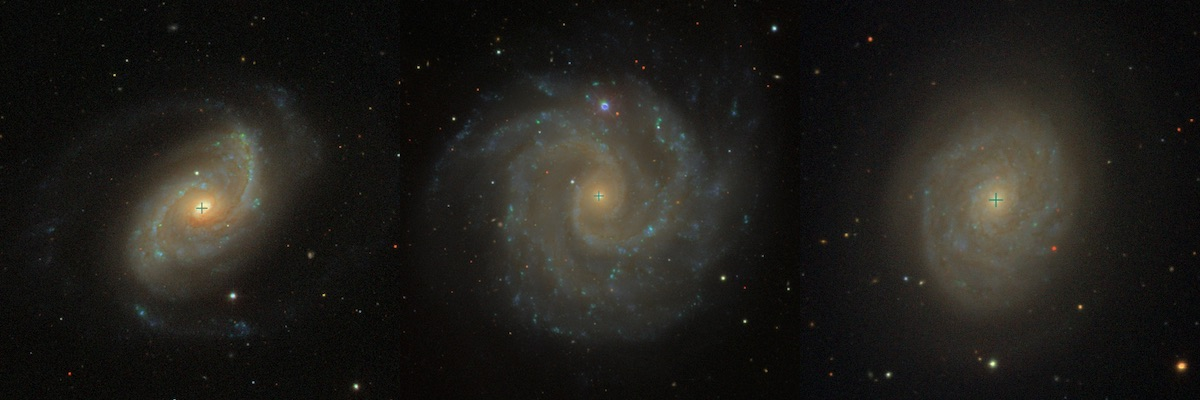
\includegraphics[width=15cm]{plots/galaxy_types.jpg}
  \caption{Examples of the different types of spiral galaxy present in the sky. The left column shows the \textbf{grand design spiral NGC 5248}, the middle shows the \textbf{many-armed spiral NGC-3184} and the right shows the \textbf{flocculent spiral NGC-4689}. Images were taken with the Sloan Digital Sky Survey Telescope.}
  \label{fig:spiral-galaxy-types}
\end{figure*}

\textbf{
Whatever kind of spiral is present in a disc galaxy, there is plenty of evidence to suggest that they have a significant role on the overall evolution of that galaxy. For example, a majority of the population of young stars in a galaxy are located in its spiral arms \citep{2011EAS....51...19E}, and there is evidence that spiral arms may trigger star formation \citep{2013A&A...560A..59C} perhaps via their ability to promote the growth of Giant Molecular Clouds \citep{2014IAUS..298..221D}. The rearrangement of disc gas and stars driven by spiral arms (e.g. \citealt{2018MNRAS.476.1561D}) may lead to the formation of disc-like bulges (commonly called ``pseudobulges''; e.g. \citealt{2004ARA&A..42..603K}), which are prevalent in most spiral galaxies, including those without bars \citep{2010ApJ...716..942F}. Studies of spiral morphology have also found interesting correlations with other galactic properties, such as a correlation between the tightness of spiral arms and central mass concentration (\citealt{2019ApJ...871..194Y}, though neither \citealt{2017MNRAS.472.2263H} nor \citealt{2019MNRAS.487.1808M} found such a relation in large samples). Spiral tightness is also observed to correlate with with rotation curve shape (\citealt{2005MNRAS.359.1065S}), with rising rotation curves creating more open spiral structure. These predictions and observations provide compelling reasons for continued investigation of the underlying rules and dynamics of spiral structure, as doing so is essential for understanding the secular evolution of disc galaxies.
}

Our current understanding of the mechanisms which drive spiral growth and evolution suggests that different forms of spiral arms in a galaxy may be triggered by different processes. Grand design spirals are thought to have undergone a tidal interaction \citep{2010MNRAS.403..625D,2017ApJ...834....7S}, be driven by a bar (as seen in gas simulations, \citealt{1976ApJ...209...53S,2008A&A...489..115R}, and suggested for stars by Manifold theory, \citealt{2006A&A...453...39R,2009MNRAS.394...67A,2009MNRAS.400.1706A}), or be obeying (quasi-stationary) density wave theory (QSDW theory), in which spiral arms are slowly evolving, ever-present structures in the disc (as first proposed by \citealt{1964ApJ...140..646L}). Flocculent spirals are thought to be formed through swing amplification (shearing of small gravitational instabilities in the disc), and be transient and recurrent in nature \citep{1966ApJ...146..810J}.

One of the fundamental assumptions of early work on spiral formation mechanisms (primarily QSDW) was that the disc of a galaxy, if unstable to spiral perturbations, would create a stable, static wave which would exist unchanged for many rotational periods \citep{1964ApJ...140..646L}. The motivation for static waves with small numbers of arms \sout{(with a preference for $m=2$)} was primarily observational: most disc galaxies observed at the time showed spiral structure with low spiral arm numbers, suggesting that spirals exist for a long time or are continually rebuilt. \textbf{This, in combination with theoretical arguments about the ``winding problem", motivated the original static density waves of \citet{1964ApJ...140..646L}, to which swing amplification was added by \citet{Toomre1981}  to provide a way to counteract the short lifetime of stellar density waves.}

More recently, simulations demonstrate that spirals do not maintain a constant tightness (often quantified by pitch angle, the angle between the spiral and the tangent to a circle centred on the galaxy, \citealt{1987gady.book.....B}, illustrated in Figure \ref{fig:pitch-angle-example}), and instead wind-up over time due to the differential rotation of the disc \citep{2013ApJ...763...46B}. Recent research suggests that spirals arms are transient, and continually dissipate and re-form \citep{2014PASA...31...35D}. These spirals can be maintained through the same mechanisms that drive QSDW spirals (i.e. ``wave amplification by stimulated emission of radiation'', \citealt{1976ApJ...205..363M}; swing amplification, \citealt{1965MNRAS.130..125G}), but do not require the idealistic disc conditions required for the formation and maintenance of a stationary wave. The pitch angles of these transient spiral arms will decrease due to the differential rotation of the disk, with the density of the arm peaking at some critical pitch angle, before dissipating to be reformed.

\begin{figure}
  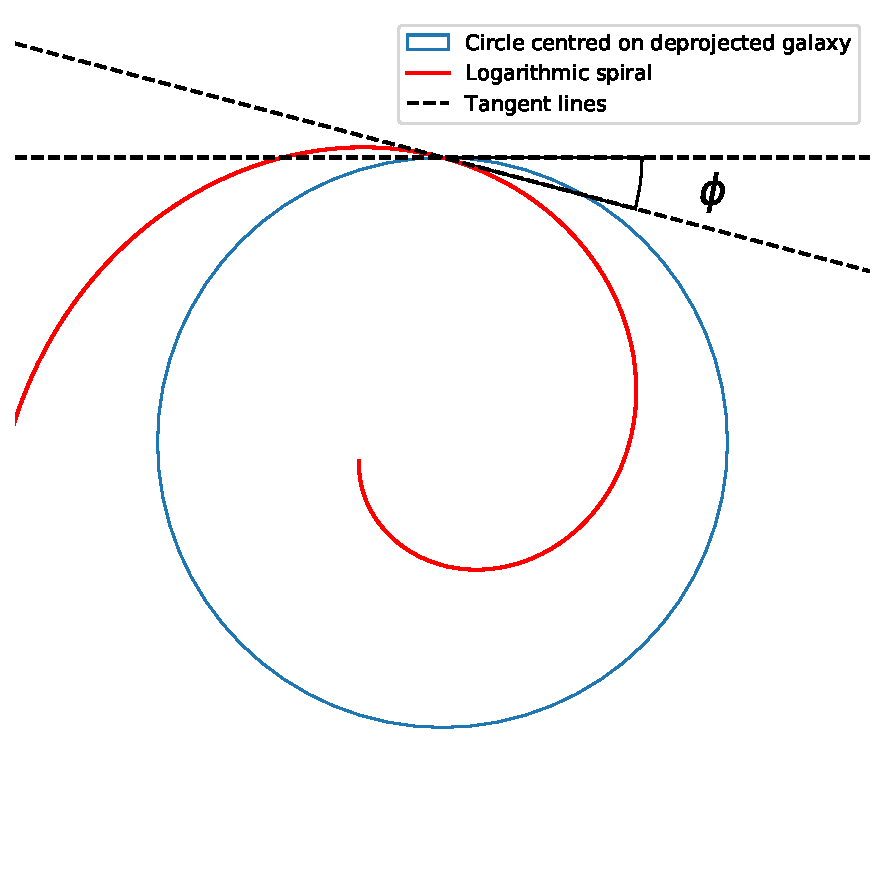
\includegraphics[width=8.4cm]{plots/pitch-angle-explanation.pdf}
  \caption{Illustration of the definition of pitch angle. It is given as $\phi = \tan^{-1}\left(\frac{\mathrm{d}r}{\mathrm{d}\theta}\ /\ r\right)$, or the angle between the spiral (red) and the tangent to a circle centred on the galaxy (blue).}
  \label{fig:pitch-angle-example}
\end{figure}

In this dynamic picture of spiral arms, pitch angle monotonically decreases from a spiral arm's formation to its dissipation. As a particular example of this, \citet{2019arXiv190910291P} propose a simple test of the winding of spiral arms, predicting that the cotangent of the pitch angle of a spiral arm ($\cot \phi$) evolves linearly with time. They found that the distribution of pitch angles of their sample of 86 galaxies was consistent with this prediction, which they present as evidence against QSDW theory in favour of the dynamic spirals produced in many simulations.

We aim to test this idea of spiral winding using data from the \textit{Galaxy Builder} citizen science project for the spiral galaxies present in \citet{2020arXiv200610450L}. We make use of Bayesian hierarchical modelling to measure galaxy pitch angle from the spiral arms produced by \textit{Galaxy Builder}. This methodology allows us to quantify the differences in pitch angles between arms in a single galaxy, as well as investigate the distribution of pitch angles in the galaxy population and investigate relationships between pitch angle and galaxy morphology.

Using Galaxy Zoo 2 data \citep{Willett2013:1308.3496v2} we further separate of galaxies by the presence and strength of a stellar bar. This will allow us to test simulations of gas in barred galaxies, which often demonstrate that bars can drive long-term spiral evolution \citep{2008A&A...489..115R}, or boost transient spiral structure \citep{2012MNRAS.426..167G}. Manifold theory \citealt{2006A&A...453...39R,2009MNRAS.394...67A,2009MNRAS.400.1706A} is one attempt to determine the orbits of stars in bar-driven spiral arms: it proposes that stars in the vicinity of the unstable Lagrangian points at either end of the bar tend to escape along predictable orbits, governed by invariant manifolds. One of the primary factors influencing the shape of this invariant manifold is the relative strength of the non-axisymmetric forcing caused by the bar, with stronger bars resulting in spirals with larger pitch angles.

Many other galactic components may correlate with spiral morphology, including bulge fraction (\citealt{1975A&A....44..363Y}, \citealt{2013MNRAS.436.1074S}, \citealt{2019MNRAS.487.1808M}) and black hole mass (\citealt{2008ApJ...678L..93S}, \citealt{2017MNRAS.471.2187D}, \citealt{2019MS&E..571a2118A}). Larger bulges and more massive central black holes have both \textbf{been observed to} correlate with more tightly wound spiral arms. \textbf{We can also test this with the data presented in this paper.}

\textbf{This paper is structured as follows: In Section \ref{section:method} we introduce methods to measure galaxy pitch angle, and present our sample, and our Bayseian hierarchical modeling method making use of \textit{Galaxy Builder} to estimate galaxy and population pitch angles. Section \ref{section:constraints-on-galaxy-phi} presents our general constraints on pitch angles in our section, while} Section \ref{section:morphology-comparison} examines the correlation between pitch angle and bulge size implied by the Hubble sequence, and pitch angle and bar strength implied by Manifold theory. Section \ref{section:spiral_winding} investigates spiral arm winding using the test derived by \cite{2019arXiv190910291P} (uniformity of galaxy pitch angle in $\cot\;\phi$). \textbf{We provide a summary and conclusions in Section \ref{section:summary}.}  Where necessary, we make use of $H_0 = 70\ \text{km}\ \text{s}^{-1}\ \text{Mpc}^{-1}$.
